\documentclass[conference]{IEEEtran}
\IEEEoverridecommandlockouts
% The preceding line is only needed to identify funding in the first footnote. If that is unneeded, please comment it out.
\usepackage{cite}
\usepackage{url}
\usepackage{amsmath,amssymb,amsfonts}
\usepackage{algorithmic}
\usepackage{graphicx}
\usepackage{textcomp}
\usepackage{xcolor}
\usepackage{titling}
\def\BibTeX{{\rm B\kern-.05em{\sc i\kern-.025em b}\kern-.08em
    T\kern-.1667em\lower.7ex\hbox{E}\kern-.125emX}}
\begin{document}


\title{
  Analyzing and Predicting League of Legend's Game Outcome using PySpark and it's Machine Learning Models
  }
  
\author{% 
Janam Patel \\ 
College of Computing and Informatics\\
Drexel University, Philadelphia, PA 19104, USA}

\maketitle

\begin{abstract}
League of Legends (LOL) is one of the biggest Esports games in the world [1], with over 180 million active players [2]. In this study, we want to analyze and predict the game outcome for big tournaments held by Riot Games between the years 2014-2018. We use $PySpark$’s built-in functionality to do some explanatory data analysis, and then also use built-in ML models like Logistic Regression, Random Forest, and Decision Tree models to predict the game outcome. We also used PySpark with $SkLearn$’s GridSearch, which is different from when we use it with $Numpy$ or $Pandas$. Surprisingly, the model performed well with over 91\% accuracy.\\  
\end{abstract}

\begin{IEEEkeywords}
PySpark, League of Legends, LOL, Esports, Logistic Regression Classifier, Random Forest Classifier, Decision Tree Classifier, SkLearn, GridSearchCV, Pandas, Numpy
\end{IEEEkeywords}

\section{Introduction}
Every year Riot Games hold the League of Legends' Championship Tournament in September. Where teams from all over the world come to compete for the title of World Champions. The tournament is watched by 100 million viewers from all over the world [3], for comparison, NBA's highest viewership was 36 million was back in 1998. The price pool from 2018 had exceeded 6 million dollars, which is divided between five-player [3]. Though teams have different strategies to win each game, the main play style of the game stays the same, which is earning gold, killing opponents, denying opponents from getting ahead in terms of levels, and closing out the game before the opponent team is able to react and overturn the game. We'll be using PySpark to analyze game stats and also, use the data to train models on different classification models to determine the outcome of the game. 

\section{LOL Dataset}
The League of Legends (LOL) dataset from Kaggle [4] consists of all the professional games from years 2014 to 2018. The dataset was obtained through the website of match history which used to be maintained by Riot Games but is now discontinued. Since the website was maintained by the Riot Games, the same company that organizes these events and the creator of the game, we don't have to question the data integrity. Each row consists of different attributes of the game and its outcome. The target variable is Winner which has values of 0, and 1. 0 being the Win and 1 being loss. The two teams playing are representing blue and red, depending on the side of the map they choose to play on. The dataset has a total of 19 different attributes and 7620 samples.


\begin{table}[!ht]
    \begin{tabular}{|| l | l ||}
        \hline
        \\[-1em]
        \textbf{Columns} & \textbf{Description} \\
        \hline\hline
        \\[-1em]
        League & League or Tournament the match took place in\\
        \hline
        \\[-1em]
        blueTeamTag & Blue Team's tag name (ex. Team SoloMid is TSM)\\
        \hline
        \\[-1em]
        redTeamTag & Red Team's Tag Name (ex. Team SoloMid is TSM)\\
        \hline
        \\[-1em]
        gamelength & Game length in minutes\\
        \hline
        \\[-1em]
        goldblue & Blue Team's Final Total Gold\\
        \hline
        \\[-1em]
        bKills & Number of Kills by Blue Team\\
        \hline
        \\[-1em]
        bTowers & Number of towers destroyed by Blue Team\\
        \hline
        \\[-1em]
        bInhibs & Number of inhibitor destroyed by Blue Team \\
        \hline
        \\[-1em]
        bDragons & Number of dragon by Blue Team\\
        \hline
        \\[-1em]
        bBarons & Number of baron nashor by Blue Team\\
        \hline
        \\[-1em]
        bHeralds & Number of rift herald by Blue Team\\
        \hline
        \\[-1em]
        goldred & Red Team's Final Total Gold\\
        \hline
        \\[-1em]
        rKills & Number of Kills by Red Team\\
        \hline
        \\[-1em]
        rTowers & Number of towers destroyed by Red Team\\
        \hline
        \\[-1em]
        rInhibs & Number of inhibitor destroyed by Red Team \\
        \hline
        \\[-1em]
        rDragons & Number of dragon by Red Team\\
        \hline
        \\[-1em]
        rBarons & Number of baron nashor by Red Team\\
        \hline
        \\[-1em]
        rHeralds & Number of rift herald by Red Team\\
        \hline
        \\[-1em]
        Winner & Win(0) or lose(1)\\    
        \hline
    \end{tabular}
    \\[1em]
    \caption{Dataset Attributes Description}
    \label{table:1}
\end{table}
    
\section{\textbf{Exploratory Data Analysis}}
For analysis, I sought to answer the following questions:

\begin{enumerate}
    \item Key Insights on the data provided by Pandas Profiling?
    \item Which side of the map has the most number of wins?
    \item On which side of the map, do teams earn more gold?
    \item Is there big difference in kill and objective count when Team plays on a specific side?
    \item What is the probability of game lasting for 30 or more minutes?
    \item Number of Games played and won by each League? Do teams from that league appear more often in tournaments?
\end{enumerate}

From the report generated using Pandas Profiling, the main thing I want to point out is that we don't have any null values. We learn that there is a high correlation between, goldred and goldblue with gamelength (fig. 1). This is understandable since players gain gold by killing opponents, killing monsters, taking objectives, and also generating 20.4 gold every 10 seconds passively. Report also tells us that rKills, bKills, Blue Total Objective, and Red Total Objective have a high number of 0's. Although having zeros isn't bad for this datatset, this isn't looking good for any team's stats for that game. Usually, when these attributes are 0 for a team, it means that the opposing team dominated and won the game very easily.

\begin{figure}[!ht]
  \begin{center}
 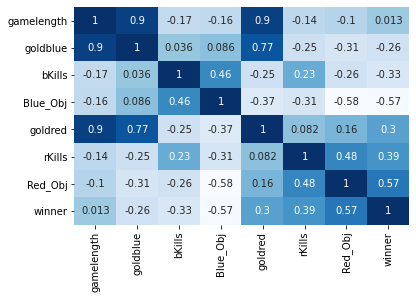
\includegraphics[height=6cm]{graphics/corr.png}
 \caption{Heatmap Correlation of the Data}
 \label{Heatmap Correlation of the Data}
 \end{center}
\end{figure}

In each game, the teams play on a symmetrical, square map with one team starting the other starting on the bottom left as the Blue team and on the top right as the Red team (fig. 2). The goal is to push the lanes where players destroy turrets and inhibitors and create pressure to win the lane and eventually the game.

\begin{figure}[!ht]
  \begin{center}
 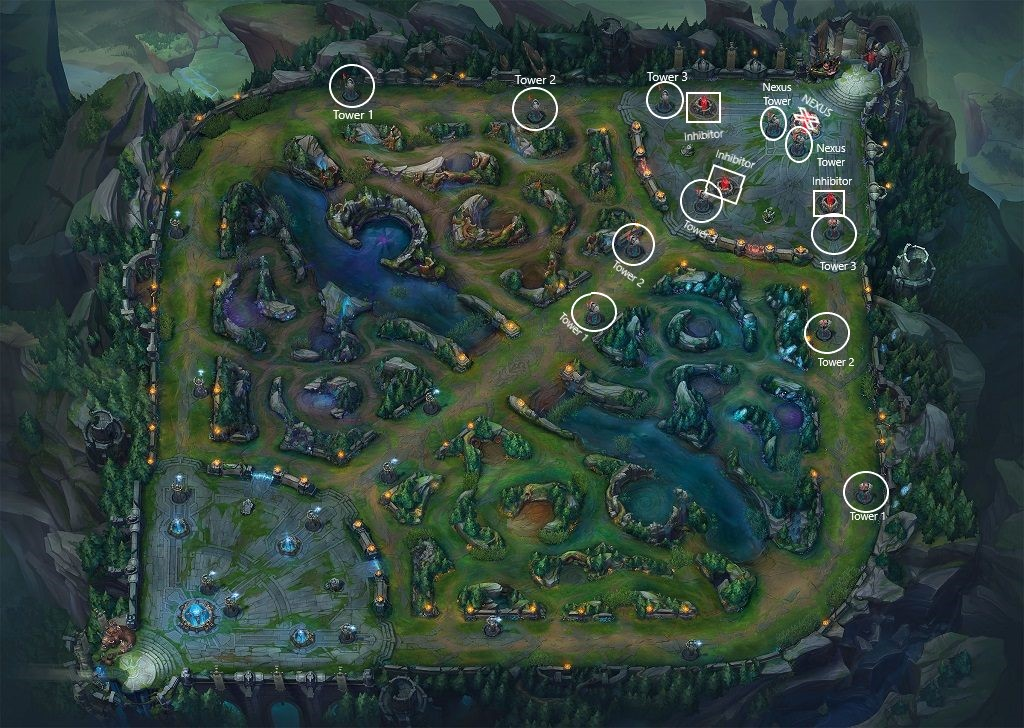
\includegraphics[height=6cm]{graphics/map.jpg}
 \caption{Game Map}
 \label{Game Map}
 \end{center}
\end{figure}

Usually, in team-oriented games, the maps are designed in a way where no one team has an advantage over the other, and that is also true for this map. But with its unique design of sides being assigned to the corner of each side, players on the red side will tend to struggle if the players preferred playstyle is playing with a locked screen, where the screen is locked over the champions movement, compared to a free screen where your screen isn't locked onto champion and players have to push the mouse around to try and look around the map. 

\begin{figure}[!ht]
  \begin{center}
 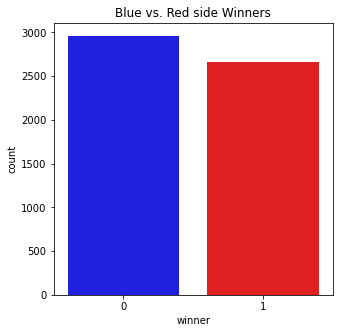
\includegraphics[height=6cm]{graphics/BvR_w.png}
 \caption{Game Map}
 \label{Waveform of each emotion}
 \end{center}
\end{figure}

In fig. 3 we see that the Blue side has approximately 400 more wins compared to the Red side. Though the map is symmetrical, the red side does seem a little hard to play when you have a screen lock on. Screen lock is especially a standard when there are team fights so players' play style has a high impact on the game outcome since players have different comfort play styles. So, we notice that there's some advantage when playing on the blue side. Are there other factors that are affected when playing on a specific side of the map? So, let's see on which side do teams end the game with more team gold. We first check the top-five team with gold earned on the blue side then based on those top-five teams, we check the same teams' gold count on the red side and see how they compare.

\begin{figure}[!ht]
  \begin{center}
 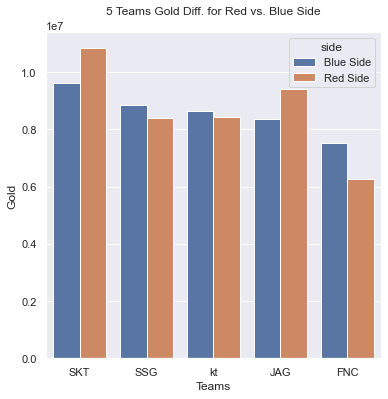
\includegraphics[height=6cm]{graphics/gold_diff_RvB.png}
 \caption{Top 5 team Gold Comparison based on the Map Side}
 \label{Top 5 team Gold Comparison based on the Map Side}
 \end{center}
\end{figure}

We see that the only team who earned more gold on the red side is SKT and JAG. It's not surprising to see SKT since they are the only team that has won the World Championship three times [5]. How does the gold compare overall?

\begin{figure}[!ht]
  \begin{center}
 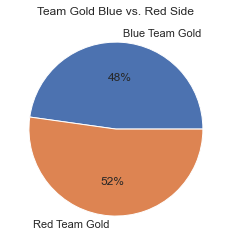
\includegraphics[height=6cm]{graphics/BvR_g.png}
 \caption{Blue vs. Red Side Team Gold Comparison}
 \label{Blue vs. Red Side Team Gold Comparison}
 \end{center}

%\begin{figure}[!ht]
  \begin{center}
 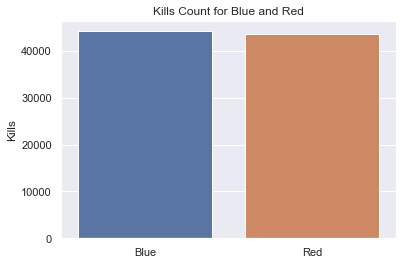
\includegraphics[height=5.3cm]{graphics/Kills.png}
 \caption{Kills Count for Blue and Red}
 \label{Kills Count for Blue and Red}
 \end{center}
%\end{figure}

%\begin{figure}[!ht]
  \begin{center}
 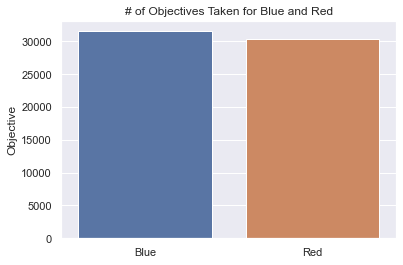
\includegraphics[height=5.5cm]{graphics/obj.png}
 \caption{ Number of Objectives Taken for Blue and Red}
 \label{Number of Objectives Taken for Blue and Red}
 \end{center}
\end{figure}

Based on fig. 5, teams earn more gold on the red side compared to the blue side. So, it's a good thing that the professional players are not affected by the standard and minor things like picking the right or good side of the map and knowing how to play on both sides of the map. According to fig. 6 and 7 teams on both sides of the maps have approximately the same kill count and number of objectives taken. Overall, this proves that map is designed fairly and there is very little advantage on playing on the blue side, its so little that it probably won't affect the game outcome heavily. 

\begin{figure}[!ht]
  \begin{center}
 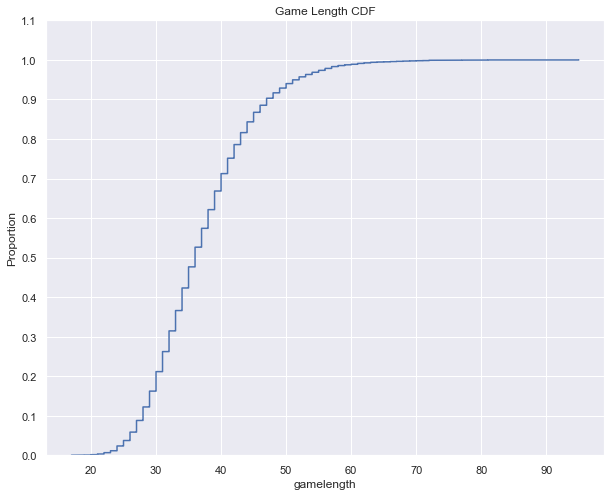
\includegraphics[height=6cm]{graphics/cdf.png}
 \caption{Game Length CDF}
 \label{Game Length CDF}
 \end{center}
\end{figure}

In League of Legends, the team is only allowed to surrender after 20 minutes mark which requires four of five votes to forfeit the game. In a professional tournament, forfeiting a game is rare since it's a professional game, a small mistake by a player could easily let the opponent punish the action and try and overturn the game. Looking at fig. 8, we notice that only 10\% of games end before 30 minutes mark, but also 10\% of games lasts for more than 50 minutes as well. 90\% of the games last up to 50 minutes. Professional games ending before 30 minutes mark usually result in one of the teams dominating the early game and just slowly increasing their lead to eventually close out the game before the opponent can find a chance to overturn the game. \\

Between 2014-2018, there were a total of 15 different Leagues around the world with each consisting different number of teams. Over the years the Leagues have either merged or were shut down with the current number of Leagues being 12 as of 2020 [6]. As you can see in fig. 9, LCK had the highest number of games won with over 600 games between the years 2014-2018. In fig. 10, we see that out of the top 10 teams by win count, four are from LCK. That would explain why LCK had such high win counts compared to the other Leagues. SKT, the three-time world champions, and the world's best player, Lee Sang-hyeok, better known as Faker are from LCK [7]. SSG hold one world champion title, JAG and KT have been the runner ups few times who also belong to LCK.

\begin{figure}[!ht]
  \begin{center}
 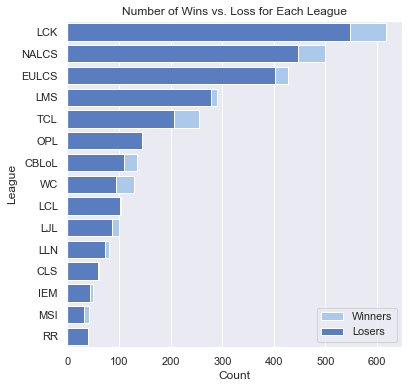
\includegraphics[height=6cm]{graphics/win_v_loss.png}
 \caption{Wins vs. Loss for Each League}
 \label{Wins vs. Loss for Each League}
 \end{center}
	
  \begin{center}
 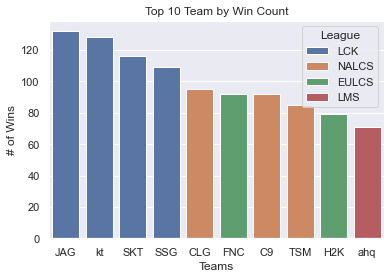
\includegraphics[height=6cm]{graphics/teams_win.png}
 \caption{Top 10 Team by Win Count}
 \label{Top 10 Team by Win Count}
 \end{center}
\end{figure}

\section{Machine Learning}
\subsection{PySpark}
This section primarily covers our work that was done by PySpark's built-in Machine Learning. Our data will use the following attributes: gamelength, goldblue, bKills, bTowers, bInhibs, bDragons, bBarons, bHeralds, goldred, rKills, rTowers, rInhibs, rDragons, rBarons, rHeralds, to predict our "Winner" variable. We use VectorAssembler to transform our attributes columns into a single vector column. We split the dataset by keeping 80\% of it for training and res for testing data, with the seed set to 42 to ensure the same results on each run of the code. Since it's a classification problem, we'll use Logistic Regression, Random Forest Classifier,  and Decision Tree Classifier models to train and test our data.\\

\begin{figure}[!ht]
  \begin{center}
 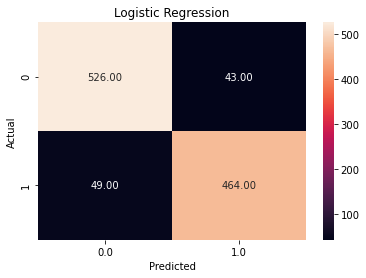
\includegraphics[height=6cm]{graphics/lr_cm.png}
 \caption{Logistic Regression Confusion Matrix}
 \label{Logistic Regression Confusion Matrix}
 \end{center}
\end{figure}

\begin{figure}[!ht]
  \begin{center}
 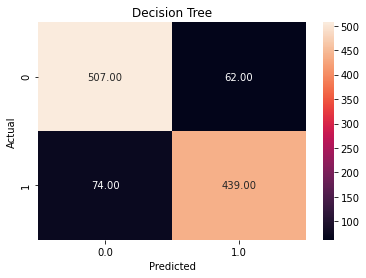
\includegraphics[height=6cm]{graphics/dt_cm.png}
 \caption{Decision Tree Confusion Matrix}
 \label{Decision Tree Confusion Matrix}
 \end{center}
\end{figure}

\begin{figure}[!ht]
  \begin{center}
 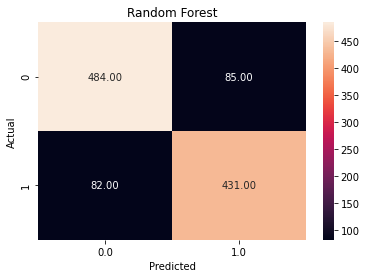
\includegraphics[height=6cm]{graphics/rf_cm.png}
 \caption{Random Forest Confusion Matrix}
 \label{Random Forest Confusion Matrix}
 \end{center}
\end{figure}

For each of the models, currently, the hyperparameters were kept at default. Our Logistic Regression had an accuracy of 91.50\% for our testing dataset, which is great. Fig. 11, which is Confusion Matrix of Logistic Regression, shows that only 92 out of 1082 testing samples were predicted to be incorrect. Decision Tree had accuracy of 87.43\% followed by Random Forest with the accuracy of 84.94\%. Fig. 12 and fig 13 show the confusion matrix of Decision Tree and Random Forest. As seen in fig 14. the ROC curve proves that our model is working and is accurate.

\begin{figure}[!ht]
  \begin{center}
 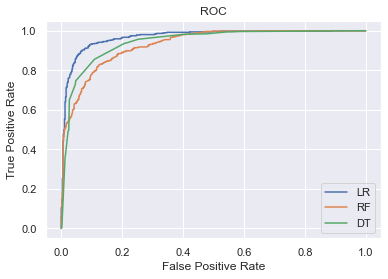
\includegraphics[height=6cm]{graphics/roc.png}
 \caption{ROC}
 \label{ROC}
 \end{center}
\end{figure}

\subsection{SkLearn's GridSearch}
We know that Sklearn has this great tool called GridSearch which goes through all the possibilities for the model hyperparameter tuning to give you the best result. But this doesn't work properly with the PySpark data frame which has featured in the vector form. So, to use GridSearch with PySpark Dataframe, we would keep the columns as is instead of transforming them into vectors. We'll also need to replicate each record for n number of times. When we have a cluster with n number of nodes, the GridSearch will be n times faster depending on the number of nodes available to use [9]. I personally didn't have access to the proper cluster so I didn't see much change in speed for computation but when run on a proper cluster, you will see a significant difference. 

\begin{figure}[!ht]
  \begin{center}
 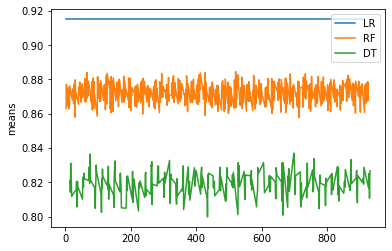
\includegraphics[height=5cm]{graphics/grid.png}
 \caption{Grid Search}
 \label{Grid Search}
 \end{center}
\end{figure}

As you can see from fig. 15, Logistic Regression performed best again with almost 92\% accuracy, but Random Forest did 2nd best followed by the Decision Tree, which is opposite from when we use it in PySpark. It could be because for PySpark we didn't do any hyperparameter tuning, but for GridSearch we did. 


\section{Conclusion}
Overall, Logistic Regression was the Best performing model with over 91\% accuracy. Random Forest and Decision Tree did pretty well as well, and maybe there are possibilities of those models to do better if we do some hyperparameter tuning. 
We can use this analysis and model to come up with a new strategy and find which champion has a higher chance of winning based on the ability that the champion provides. More importantly, team and coaching staff can see which player is performing well and which player is underperforming allowing them to make changes to the team roster. This not only benefits teams but also players as they'll want a comfortable team and strategy to work with where they truly shine and put on a good fight in each game. 


\section{Future Scope}
We got a good accuracy score just from some data points, now if we used whole proper dataset, where we had champion names, player names, player stats, time on each event, and time at which objectives were taken, then we can use this model and analysis to change and update strategy as the game updates and adapts to new play style.

\begin{thebibliography}{00}


\bibitem{1} “The most popular esports tournaments and leagues in 2020.” [Online]. Available: https://escharts.com/blog/most-popular-tournaments-and-leagues-2020. [Accessed: 06-Mar-2022]. 
\bibitem{2} Facebook.com/ivanlovremarusic, “How many people league of legends in 2022? (March),” LeagueFeed, 05-Mar-2022. [Online]. Available: https://leaguefeed.net/did-you-know-total-league-of-legends-player-count-updated/. [Accessed: 05-Mar-2022]. 
\bibitem{3} A. Goslin, “The 2018 League of Legends World Finals had nearly 100 million viewers,” The Rift Herald, 11-Dec-2018. [Online]. Available: https://www.riftherald.com/2018/12/11/18136237/riot-2018-league-of-legends-world-finals-viewers-prize-pool. [Accessed: 05-Mar-2022]. 

\bibitem{4}C. Ephron, “League of Legends,” Kaggle, 24-May-2017. [Online]. Available: https://www.kaggle.com/chuckephron/leagueoflegends/version/5. [Accessed: 05-Mar-2022]. 

\bibitem{5} “SK telecom T1” Leaguepedia | League of Legends Esports Wiki. [Online]. Available: https://lol.fandom.com/wiki/SK\_Telecom\_T1?so=search. [Accessed: 05-Mar-2022]. 
\bibitem{6} “Regional Leagues,” League of Legends Esports Media Center - Regional Leagues - Assets. [Online]. Available: https://www.lolesportsmedia.com/Regional-Leagues. [Accessed: 05-Mar-2022]. 
\bibitem{7} “Faker,” Leaguepedia | League of Legends Esports Wiki. [Online]. Available: https://lol.fandom.com/wiki/Faker. [Accessed: 05-Mar-2022]. 
\bibitem{8} A. Ross, “Pyspark extract ROC curve?,” Stack Overflow, 01-Sep-1966. [Online]. Available: https://stackoverflow.com/questions/52847408/pyspark-extract-roc-curve. [Accessed: 05-Mar-2022]. 
\bibitem{9} R. Agarwal, “100x faster hyperparameter search framework with Pyspark,” Medium, 02-Feb-2020. [Online]. Available: https://towardsdatascience.com/100x-faster-randomized-hyperparameter-searching-framework-with-pyspark-4de19e44f5e6. [Accessed: 06-Mar-2022]. 

\end{thebibliography}


\end{document}
